\documentclass{beamer}
\usetheme{Madrid}
\usepackage{amsmath, amssymb}
\usepackage{pgfplots}
\pgfplotsset{compat=1.18}
\usepackage{enumerate}

\title[Max Cycle Inventory]{2.0.20}
\author{Darsh Pankaj Gajare --- EE25BTECH11020}
\date{}

\begin{document}

\begin{frame}
  \titlepage
\end{frame}

%----------- Problem Statement -----------
\begin{frame}{Question}
A manufacturing system with a production rate p units/day experiences a demand rate
of d units/day where $p \geq d$. Let Q be the maximum production quantity per period.
When the total production in a period reaches Q units, the production is stopped and
restarted only when inventory becomes zero. In such a scenario, the maximum cycle
inventory is \hfill (2007 PI)
\begin{enumerate}
\item $Q \cdot p \cdot (p - d)$ \qquad
\item $\dfrac{Q}{(p-d)^p}$ \qquad
\item $\dfrac{Q}{p}(p - d)$ \qquad
\item $\dfrac{p(p-d)}{Q}$
\end{enumerate}
\end{frame}
%----------- Derivation -----------
\begin{frame}{Derivation}
  \begin{block}{Step 1: Production phase duration $t_p$}
    Total production in one cycle equals $Q$ at rate $p$:
    \[
      t_p = \frac{Q}{p}
    \]
  \end{block}
  \begin{block}{Step 2: Net inventory build-up during $t_p$}
    Inventory rises at rate $(p - d)$ during production:
    \[
      I_{\max} = (p - d) \times t_p
    \]
  \end{block}
  \begin{block}{Step 3: Final result}
    \[
      \boxed{I_{\max} = \frac{Q}{p}(p - d)}
    \]
  \end{block}
\end{frame}

%----------- Answer -----------
\begin{frame}{Answer}

  \begin{alertblock}{Answer: Option (c)}
    \[
      I_{\max} = \frac{Q}{p}(p - d)
    \]
  \end{alertblock}
\end{frame}
\begin{frame}{Inventory Profile}
  \begin{figure}
    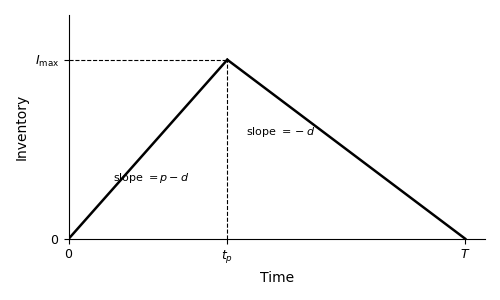
\includegraphics{figs/inventory.png}
  \end{figure}
\end{frame}
\end{document}
